\documentclass[10pt]{article}
\usepackage{float}
\usepackage{listings}
\usepackage[french]{babel}
\usepackage[utf8x]{inputenc}
\usepackage{subcaption}
\usepackage{listings}
\usepackage{wrapfig}
\usepackage{color}
\usepackage{amsmath}
\usepackage{amsfonts}
\usepackage{mathtools}
\usepackage{graphicx}
\usepackage{caption}
\definecolor{dkgreen}{rgb}{0,0.6,0}
\definecolor{gray}{rgb}{0.5,0.5,0.5}
\definecolor{mauve}{rgb}{0.58,0,0.82}
%opening

\lstset
{frame=tb,
	language=R,
	aboveskip=3mm,
	belowskip=3mm,
	showstringspaces=false,
	framexleftmargin=5mm,
	columns= fixed,
	numbers = left,
	basicstyle={\small\ttfamily},	
	numberstyle=\tiny\color{gray},
	keywordstyle=\color{blue},
	commentstyle=\color{dkgreen},
	stringstyle=\color{mauve},
	breaklines=true,
	breakatwhitespace=true,
	tabsize=3
}


\title{
	\normalfont \normalsize 
	\textsc{Université de Technologie de Compiègne\\ 
		SY09:Analyse des données et Data-Mining , P17} \\
	[10pt] 
	\rule{\linewidth}{0.5pt} \\[6pt] 
	\huge Rendu TP2\\
	\rule{\linewidth}{2pt}  \\[10pt]
}
\author{Oumaima Talouka, Zineb Slam}
\date{\normalsize \today}

\begin{document}
	{\let\newpage\relax\maketitle}	
	
		Dans ce TP2 nous allons travailler sur la méthode de classification automatique qui est une  méthode non supervisée, c'est a dire on a aucune connaissance a priori ni sur le nombre ni sur le nom des classes qui peuvent exister. Nous utiliserons en majorité la méthode des \textbf{kmeans} dont nous analyserons et critiquerons les résultats
	
	\section{ Exercice 1: Visualisation des données}
	Nous disposons de 3 jeux de données:  \textbf{Iris}, \textbf{Crabs} et une jeu de données \textbf{Mutations} de dissimilarites des espèces
	
	\subsection{Iris}
		Les iris est un jeu de donnes de la librairie \textit{MASS} avec \textbf{150 individus} et 4 variables (Sepal.Length, Sepal.Width, Petal.Length et Petal.Width).  La variable Z de réponse est l'espèce. Le but est d'identifier l'espèce de chaque individu en fonction des 4 variables: .	Pour commencer nous allons centrer et réduire les données puis effectuer une ACP pour pourvoir réduire la dimension du dataset et passer de 4 dimensions et 2 dimensions. Après avoir fait appel a la fonction \textit{prcomp} nous affichons les données dans le premier plan factoriel sans tenir compte de l'espèce. Nous notons d'abord que les 2 premiers plan factoriels expliquent \textbf{95.8\%} des données \textit{(inertie expliquée}).  Ensuite  nous utilisons la fonction \textit{autoplot} pour colorer chaque espèce selon son appartenance a une espèce et ce dans le même plan factoriel.
		
	
			\begin{minipage}{.5\textwidth}
			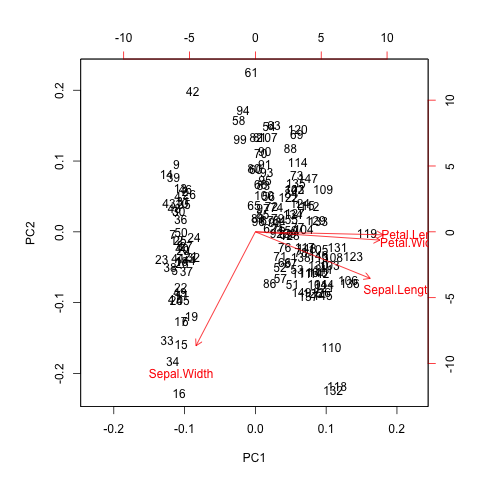
\includegraphics[width=40mm]{Figures/Iris_1/plotnospieces.png}
			\captionof{figure}{Représentation des données Iris dans les 2 premiers plan factoriel}
			\label{fig:plot_iris_nocol}
		\end{minipage}%
		\hspace{0.02\linewidth}
		\begin{minipage}{.5\textwidth}
			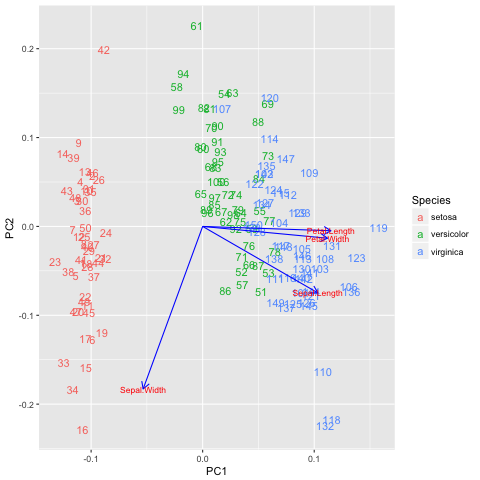
\includegraphics[width=40mm]{Figures/Iris_1/plotspieces.png}
		\captionof{figure}{Représentation des données Iris dans les 2 premiers plan factoriel en colorant les espèces}
		\label{fig:plot_iris}
		\end{minipage}
		\vspace{0.2mm}
		
	 
		Nous observons donc que selon le graphe qu'il existe au moins 2 classes bien distinctes. Maintenant nous allons faire appel a la fonction \textit{autoplot} en colorant chaque individu selon son espèce \ref{fig:plot_iris}. On constate qu'en fait il existe 3 classes: \textbf{setosa, versicolor et virginica}. Dans la première partie nous avons confondu les classes versicolor et virginica qui sont très proches et donc indistinguable a l'œil nu. L'appartenance a la classe setosa est majoritairement expliquée par la variable Sepal.Widtth, tandis que  les 2 autres classes par les 3 autres. Enfin Petal.Length et Petal.Width sont deux variables fortement corrélées On devrait donc s'attendre a 3 classes pour ce jeu de données
	
	\subsubsection{Conclusion}
	
	\subsection{Crabs}
	Nous allons procéder de la même manière que dans la question précédente mais cette fois pour les données Crabs2. Le jeu de donnes Crabs2 compte 200 individus et 4 variables \textbf{(FL2, RW2,  CL2, BD2)}  et deux variables de réponses le sexe et l'espèce Nous utilisons la fonction \textit{interaction} pour merger le sexe et l'espèce et obtenir une seule variable de réponse z. \textbf{91.2\%} des données sont expliquées par les 2 premières composantes principales. Les 2 figures ci-dessous représentent les donnes Crabs dans les 2 premiers plan factoriel sans distinguer les espèces (a gauche) puis en les colorant (a droite).
	
	
			\begin{minipage}{.5\textwidth}
		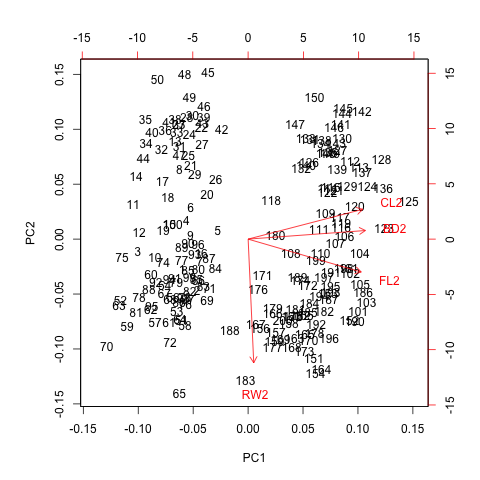
\includegraphics[width=40mm]{Figures/Crabs2_1/plotnospieces.png}
		\captionof{figure}{Représentation des données Crabs2 dans les 2 premiers plan factoriel}
		\label{fig:plot_crabs_nocol}
	\end{minipage}%
	\hspace{0.02\linewidth}
	\begin{minipage}{.5\textwidth}
		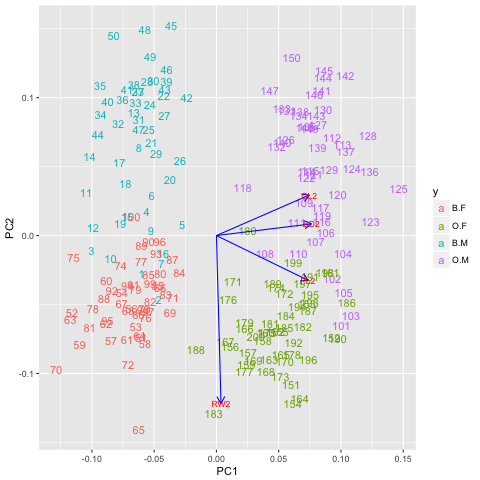
\includegraphics[width=40mm]{Figures/Crabs2_1/plotspieces.png}
		\captionof{figure}{Représentation des données Crabs2 dans les 2 premiers plan factoriel en colorant les espèces}
		\label{fig:plot_crabs}
	\end{minipage}
	\vspace{0.2mm}
	
	Selon la figure \ref{fig:plot_crabs_nocol} on peut observer qu'in existe au moins 2 classes celle de gauche et celle de droite voir 4 classes si on distingue 2 dans celle de droite et 2 dans celle de gauche. Néanmoins on peut remarquer que ces classes ne sont pas très séparées. La figure \ref{fig:plot_crabs} montre qu'il existe bien 4 classes B.F, O.F, B.M et O.M. (B et O pour distinguer les 2 espèces alors que , M et F pour le sexe) . La deuxième composante PC2 qui est concentrée dans la variable RW2 permet de distinguer le sexe, tandis que CL2, FL2, BO2 encodées dans PC1 permettent de distinguer l'espèce. On pourrait alors mettre l'hypothèse  que le fait que le sexe ne soit pas aussi distinguable que l'espèce est le fait qu'il est explique que par une seule variable tandis que l'espèce par 3.
	
	\subsubsection{Conclusion}
	Pour conclure la l'AFTD nous a permis de passer d'une representation de dissimilarites de dimension 20 a une autre de dimension 6 avec un poucentage d'inertie expliquee de 95\%. Nous n'avons pas pu choisir 2 dimensions car la representation n'est pas fiable comme les dissimilarites calculees sont loines des initiales. On peut supposer que le fait que cette methode n'a pas ete aussi performante avec ce jeu de donnes est parce que nos dissimilartites ne sont pas des  distances Euclediennes mais les differences entres les aminos acides dans les chaines chromosomique. chaque différence contribue à la distance de mutation en fonction du nombre minimum de nucléotides qui devrait être changé pour convertir l'un dans l'autre. Fitch \& Margoliash ont utilisé ces données pour construire un arbre phylogénétique.
	

	\subsection{Mutations}
	Nous disposons dans cette étude  d'une matrice de dissimilarites entre 20 individus (Homme, Singe, Kangourou, Cheval...). Grâce a la méthode \textbf{AFTD} et la fonction nous allons essayer de réduire la dimension du jeu de donnes. Nous essayerons de trouver au fur et a mesure le bon nombre de variables a choisir. Nous allons alors commencer par réduire le nombre de dimensions a 2. Pour évaluer cette représentations nous utiliserons le pourcentage d'inertie  expliquée cumulée et le  Diagramme de Shepard  Notons que dans le Diagramme de Shepard un axe représente la disimilaritee calculée pard AFTD alors que l'autre les disimmilarites initiales a partir de la matrice 20x20. Ainsi si la disimilaritee calculée par l'AFTD est exacte le Diagramme de Shepard sera une fonction y=x.
	
			\begin{minipage}{.5\textwidth}
		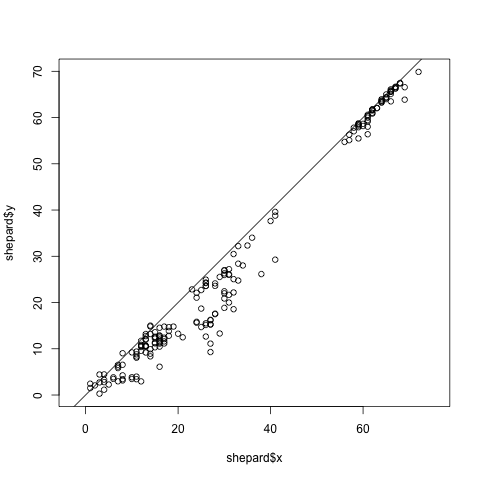
\includegraphics[width=45mm]{Figures/Mutations2_1/shepard2.png}
		\captionof{figure}{Diagramme de Shepard des Mutations avec 2 variables}
		\label{fig:shepard2}
	\end{minipage}%
	\hspace{0.02\linewidth}
	\begin{minipage}{.5\textwidth}
		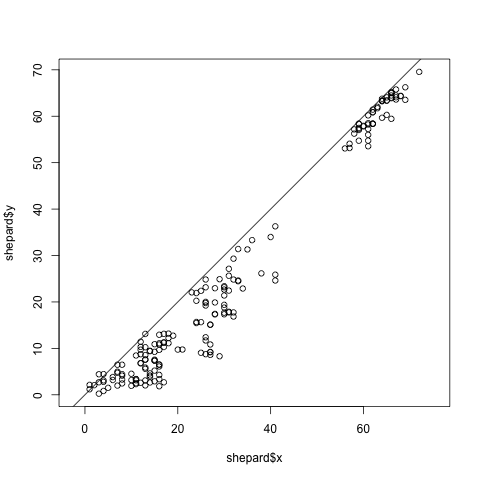
\includegraphics[width=45mm]{Figures/Mutations2_1/shepard3.png}
		\captionof{figure}{Diagramme de Shepard des Mutations avec 3 variables }
		\label{fig:shepard3}
	\end{minipage}
	\vspace{0.2mm}
	
	On remarque d'après les 2 premières présentations ci dessous que le choix de 2 variables n'est pas très représentatif de nos donnes, en effet les distances calculées par représentations en 2 dimensions restent relativement que celle de 20. Avec 3 variables il y'a plus de données les disimilarites calculées se rapprochent de leur valeur exacte mais il reste toujours d'autres points éloignés Dans la partie suivante nous allons améliorer cette représentation avec 4 puis 5 variables.s
	
		\begin{minipage}{.5\textwidth}
		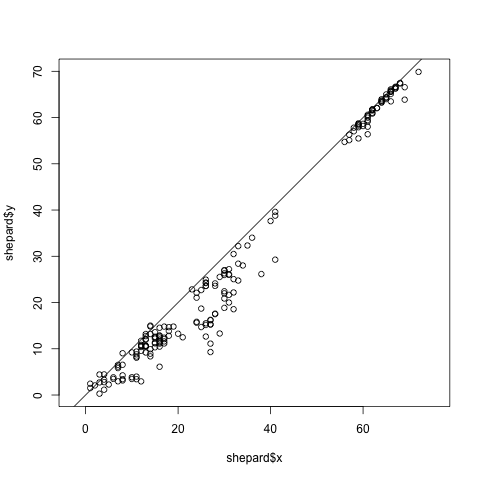
\includegraphics[width=45mm]{Figures/Mutations2_1/shepard4.png}
		\captionof{figure}{Diagramme de Shepard des Mutations avec 4 variables }
		\label{fig:shepard4}
	\end{minipage}%
	\hspace{0.02\linewidth}
	\begin{minipage}{.5\textwidth}
		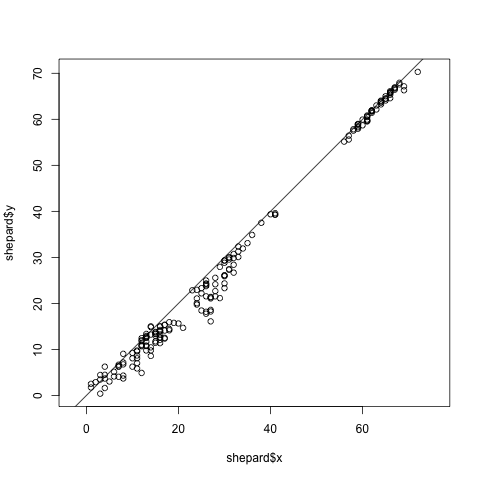
\includegraphics[width=45mm]{Figures/Mutations2_1/shepard5.png}
		\captionof{figure}{Diagramme de Shepard des Mutations avec 5 variables }
		\label{fig:shepard5}
	\end{minipage}
	\vspace{0.1mm}

	Nous remarquons que la représentation avec 4 variables le calcul de certaines disimilarites est exacte mais certaines restent loines des valeurs initiales. Avec 5 variables on se rapproche plus du cas initial ou toutes les disimilarites calculées sont plus proche de la droite y=x. Ces résultats étaient prévisibles si on calcule le pourcentage d'inertie expliquée cumule en mettant l'option \textit{eig = TRUE} dans la fonction \textit{cmscale} et récupérer les valeurs propres.
	
	\subsubsection{Conclusion}
	\begin{center}
		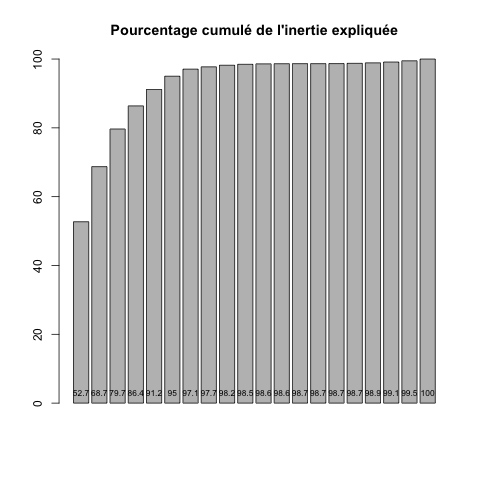
\includegraphics[width=45mm]{Figures/Mutations2_1/barplot.png}
		\captionof{figure}{Pourcentage d'inertie cumulee expliquee par AFTD}
		\label{fig:mutations_barplot}
		\end{center}
	On remarque bien qu'avec 2 variables seulement 68\%  et a partir de 4 variables le pourcentage est supérieur a 91\%.
	\section{ Exercice 2}
	\section{ Exercice 3: Méthodes des centres mobiles}
	Le but de cet exercice est de manipuler la méthode des kmeans sur les trois jeux de données Iris2, Crabs2 et mutations et analyser la qualité de la méthode et ses limites. On utilisera l'index de Rand ajustée ainsi que les représentations graphiques pour juger des performances des kmeans.
	\subsection{Iris2}
	\subsubsection{Question 1}
	Nous commençons par classifier nos méthodes en 2, 3 puis 4 classes et les représentant dans en fonction des 2 variables \textbf{Petal.Length et Sepal.Width} car comme on a vu dans lq première partie ces dernières sont bien expliquées par les 2 premières composantes principales de l'ACP.  Les résultats sont représentés ci-dessous:
	
		\begin{minipage}{.5\textwidth}
		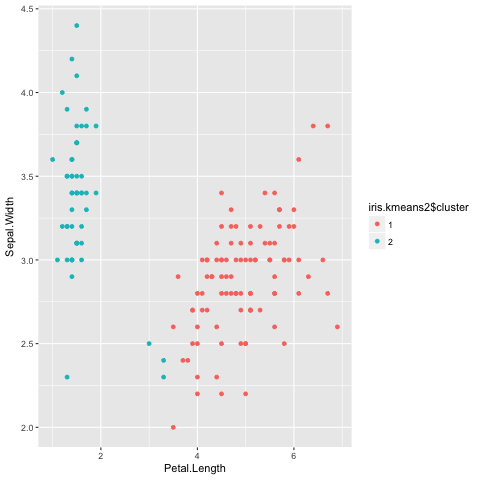
\includegraphics[width=45mm]{Figures/Iris_2/kmeans2.png}
		\captionof{figure}{Representation du jeu de donnees de Iris en 2 classes}
		\label{fig:iris_kmeans2}
	\end{minipage}%
	\hspace{0.02\linewidth}
	\begin{minipage}{.5\textwidth}
		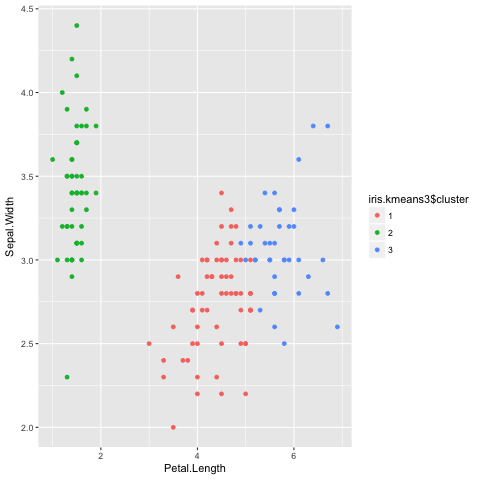
\includegraphics[width=45mm]{Figures/Iris_2/kmeans3.png}
		\captionof{figure}{Representation du jeu de donnees de Iris en 3 classes}
		\label{fig:iris_kmens3}
	\end{minipage}
	\vspace{0.1mm}
	\begin{center}
		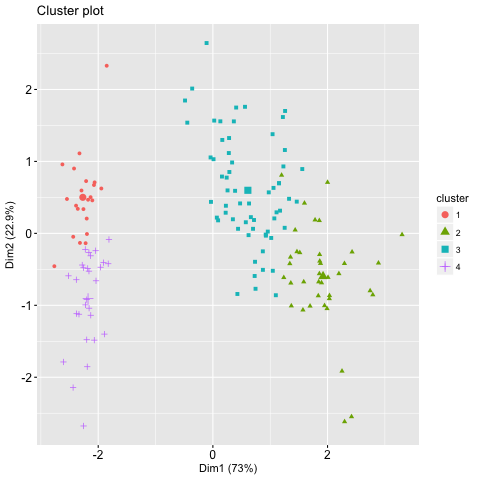
\includegraphics[width=45mm]{Figures/Iris_2/kmeans4.png}
		\captionof{figure}{Representation du jeu de donnees de Iris en 4 classes}
		\label{fig:iris_kmens4}
	\end{center}

On remarque qu'avec \textbf{k= 2 }classes nous obtenons des individus qui appartiennent a la classe 1 alors qu'ils sont plus proche de la classe 2. Tandis qu'avec \textbf{k= 3} on a des individus qui appartiennent a une classe mais qu'ils sont très éloignés La représentation avec \textbf{k= 4} classes semble plus correcte de plus avec une connaissance a priori des donnes nous savons que c'est le nombre de classe correct.\\


\subsubsection{Question 2}

A présent nous avons effectué plusieurs opérations de kmeans avec k=3, et on remarque qu'a chaque opération nous obtenons des résultats différents En effet ceci est normal car a la première itération de l'algorithme, celui ci choisit au hasard 3 points (k=3) appartenant aux individus et va construire a partir de ces points les 3 classes. Pour toujours obtenir le même résultat on peut faire un appel  au préalable a la fonction \textit{set.seed(10)} sur R.
	
\subsubsection{Question 3}	
	
Dans cette question nous cherchons a déterminer le nombre de classes minimum dans le jeu de données Iris2. Pour cela on utilise la méthode coude.  Tout d'abord on effectue 100 opérations kmeans pour chaque k = 2,3...10, en calcule l'\textit{inertie intra-classe} pour k et choisissant l'inertie minimum pour représenter l'inertie de chaque k, ce qui s'écrit comme $\hat{I_{k}} = min_{i=1..100} I_{k_{i}}$. Pour cela on utilise une matrice 10*100 ou on sauvegarde l'inertie a chaque opération puis on récupère l'inertie intra-classe minimale de chaque ligne. Le code en R détaillé et commente de cet algorithme est a trouver en annexe.
La méthode du coude consiste a choisir le point d'inflexion sur la courbe tel que l'inertie intra-classe ne diminue pas de manière aussi rapide en rajoutant des clusters.  Comme il est représenté dans la figure \ref{fig:withinvar} et comme on s'attendu aussi, le nombre de classes minimum du jeu de données Iris2 est 3. \\
	
\begin{center}
	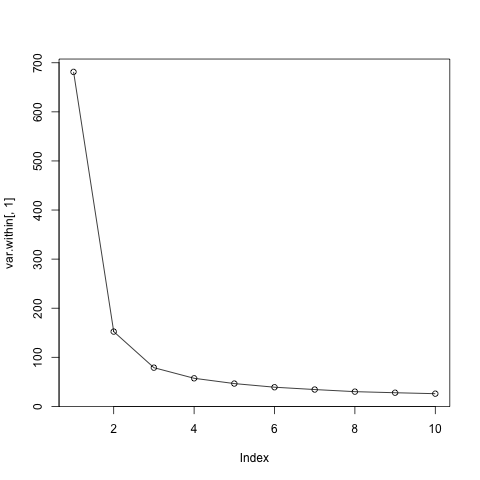
\includegraphics[width=45mm]{Figures/Iris_2/withinvar.png}
	\captionof{figure}{}
	\label{fig:withinvar}
\end{center}

 \subsubsection{ Question 4: Analyse des résultats pour k= 3}
On commence par afficher la matrice de confusion
Pour analyser la qualité de classification de la méthode des kmeans nous utilisons\textit{ l'index de Rand} ajusté et la représentation graphique. L'indexe de Rand compte le nb de paires de points qui sont classes de la même manière dans les 2 partitions. Cet indice de concordance est calculé en R grâce a la fonction \textit{adjustedRandIndex} . L'index de Rand est compris entre 0 et 1, plus l'index est proche de 1, plus la classification de la méthode correspond a la classification initiale.\\


La diagonale de la matrice de confusion représente les points qui sont bien classes. On voit donc que les individus qui appartenant a l'espèce \textit{Setosa} sont tous bien classes alors que 96\% des individus de \textit{Versicolor} ont ete mal classes et 28\% de \textit{Virginica} sont mal classes aussi.  Nous obtenons un \textbf{index de Rand= 0.73 } ce qui montre que notre classification se rapproche de la vrai classification de la colonne espèces.
Pour pourvoir comparer graphiquement les 2 classement nous avons fait une interaction entre la colonne espèce la colonne \textit{iris.kmeans\$cluster} que nous avons plot grâce a \textit{ggplot}. 

	\begin{minipage}{.5\textwidth}
		\begin{tabular}{c c c c}	
			Espece &setosa & versicolor & virginica\\
			1     &  50     &     0    &     0\\
			2     & 0       &   2      &  36\\
			3     & 0    &     48   &     14
		\end{tabular}
\end{minipage}%
\hspace{0.08\linewidth}
\begin{minipage}{.5\textwidth}
	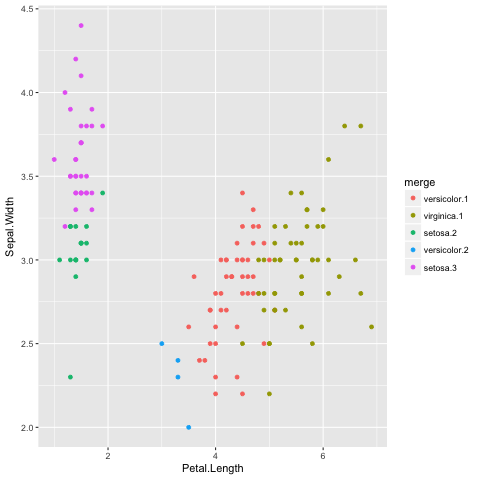
\includegraphics[width=45mm]{Figures/Iris_2/interaction.png}
	\captionof{figure}{Comparaison de la classification originale et celle des kmeans }
	\label{fig:interaction}
\end{minipage}
\vspace{0.1mm}\\

La figure \ref{fig:interaction} rejoint donc bien la remarque faite précédemment comme quoi les espèces \textit{Versicolor} er \textit{Virginica} ne sont pas bien classes. En effet ceci trouve sens si on revient a la figure \ref{fig:plot_iris}, puisqu'on voir bien que l'espèce \textit{Setosa} ne dépend que d'une seule composante PC1 tandis que les 2 autres espèces sont dépendantes des 2 et ne sont pas linéairement séparable
\subsubsection{Conclusion}
Dans cette exercice nous avons utilise la méthode des kmeans pour classifier notre jeu de données Iris. Nous retenons que cette méthode est efficace quand on a des classes bien distinctes et linéairement séparables mais cn'est pas très flexible.




\end{document}